\section{Rechenleistung}
\subsection{Aufgabenstellung}

\begin{enumerate}%Aufzählung mit Numerierung
		\item Ermitteln Sie die durchschnittliche Laufzeit einschließlich Streuung arithmetischer Grundoperationen für verschiedene vom XC-16-Compiler unterstützten Datentypen. Wie erklären Sie die Unterschiede?
		\item Berechnen Sie die ersten 10 Primzahlen, die größer als 1.000.000 (1E6) sind. Implementieren Sie denselben Algorithmus auf einem PC und vergleichen Sie die Rechenzeiten.
		
\end{enumerate}

\subsection{Lösung}
\begin{enumerate}
		\item 
		Der Programmcode wird so umgeändert wie in Listening  \ref{lst:Rechenleistung} zu sehen. Zuerst wird mit dem Oszi nur die Zeit gemessen wie lange eine LED aus ist (ohne Rechenoperation, $29,1 ns$). Anschließend kann man mit dem Oszi messen wie lange eine Grundoperation (mit Zufallszahlen) inklusiv LED ein/ausschalten benötigt. Die folgende Auflistung beinhaltet nur die Zeitdauer für die jeweilige Rechenoperation (ohne LED ein/aus).\newline
\begin{tabular}{|c|c|c|c|c|c|c|}
	\hline 
	Datentyp & Operation & Zeitdauer &  & Datentyp & Operation & Zeitdauer \\
	\hline
	
	\hline
	uint8\_t 	& + & 43,7 ns &  		& int8\_t 		& + & 57,4 ns \\ 
	\hline 
				& - & 58,1 ns &  		&  				& - & 57,4 ns \\ 
	\hline 
				& * & 72,1 ns &  		&  				& * & 71,9 ns \\ 
	\hline 
				& / & 72,5 ns &  		&  				& / & 343,9 ns \\ 
	\hline 

	%&  &  &  &  &  &  \\ %empty Line 
	\hline 
	uint16\_t 	& + & 43,4 ns &  		& int16\_t 		& + & 43,3 ns \\ 
	\hline 
				& - & 43,5 ns &  		&  				& - & 43,4 ns \\ 
	\hline 
				& * & 86,2 ns &  		&  				& * & 87,4 ns \\ 
	\hline 
				& / & 330,9 ns &  		&  				& / & 329,9 ns \\ 
	\hline

	%&  &  &  &  &  &  \\ %empty Line 
	\hline 
	uint32\_t 	& + & 115,4 ns &  		& int32\_t 		& + & 142,9 ns \\ 
	\hline 
				& - & 114,9 ns &  		&  				& - & 112,9 ns \\ 
	\hline 
				& * & 245,9 ns &  		&  				& * & 230,9 ns \\ 
	\hline 
				& / & 7,559 us &  		&  				& / & 7,95 us \\ 
	\hline

	%&  &  &  &  &  &  \\ %empty Line 
	\hline 
	uint64\_t 	& + &  &  		& int64\_t 		& + & 254,9 ns \\ 
	\hline 
				& - &  &  		&  				& - & 226,9 ns \\ 
	\hline 
				& * &  &  		&  				& * & 1,5 us \\ 
	\hline 
				& / &  &  		&  				& / & 131 us \\ 
	\hline

	%&  &  &  &  &  &  \\ %empty Line 
	\hline 
	float 	& + &  &  				& long double 		& + &  \\ 
	\hline 
			& - &  &  		&  							& - &  \\ 
	\hline 
			& * &  &  		&  							& * &  \\ 
	\hline 
			& / &  &  		&  							& / &  \\ 
	\hline  
\end{tabular} 			
\newpage

		\item Der geforderte Algorithmus ist in Listening \ref{lst:Primzahlen} abgebildet. Bei dem verfügbaren Computer (Intel Core i7 2.6GHz, 16GB RAM, 64Bit Windows 10) ergab sich eine Laufzeit von ungefähr $5 us$. (Gemessen mit CodeBlocks, $50 s$ für $10^7$ Durchläufe)
		
		Die Laufzeit des selben Programms (angepasst auf die Hardware) benötigte auf dem Mikrocontroller Board $47,8 ms$. Der Code hierzu ist in Listing \ref{lst:PrimzahlenuC} abgebildet.
		
		Damit ist der Computer ca 10.000 mal schneller als der µC.
		 ($\frac{47,8 ms}{5 us} = 9560 $, Abbildung \ref{image:scopePrimzahlen}).
\end{enumerate}

\begin{figure}[h]
	\centering
	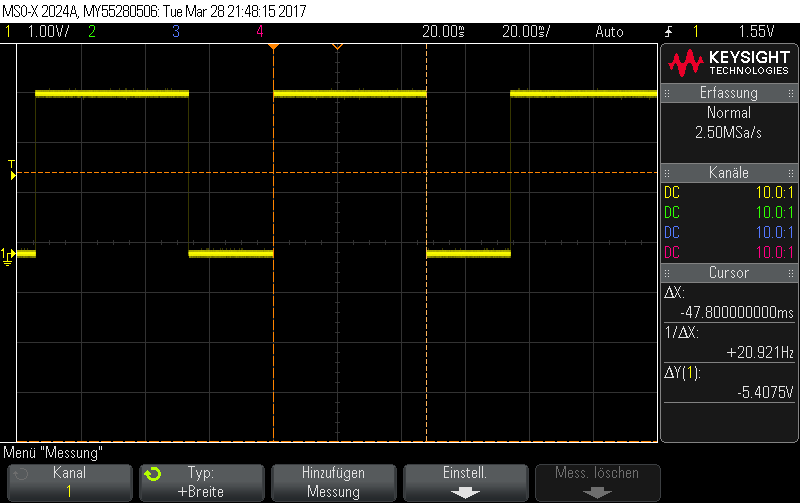
\includegraphics[width=\textwidth]{Images/scope_primzahlen}
	\caption[Laufzeit der Primzahlenberechnung]{Laufzeit der Primzahlenberechnung}
	\label{image:scopePrimzahlen}
\end{figure}

\newpage
\begin{lstlisting}[frame=htrbl, caption={Bestimmen der Rechenleistung}, label={lst:Rechenleistung}]
/* Endless Loop */
while(1){
_LED200=0;
ui8Var1 *= ui8Var2;
_LED200=1;
}//while
\end{lstlisting}

\begin{lstlisting}[frame=htrbl, caption={Algorithmus zur Berechnung der ersten 100 Primzahlen größer als 1E6}, label={lst:Primzahlen}]
#include<stdint.h>
#include<stdlib.h>
#include<math.h>

uint8_t isPrim(uint32_t ui32Number);

int main()
{
	uint32_t ui32Number= 1e6;  //start value
	uint16_t ui8PrimeCounter=0; //counts the number of calculated prime numbers
	const uint16_t ui8PrimMax=100;

	for(; ui8PrimeCounter<ui8PrimMax; ui32Number++)
		if(isPrim(ui32Number)) //check if the number is prime
		{
		//printf("%d\t%d\n",ui8PrimeCounter,ui32Number);
		ui8PrimeCounter++; //increase PrimeCounter, if the number is prime
		}
	return 0;
}
uint8_t isPrim(uint32_t ui32Number){
	uint32_t ui32Divider;
	uint32_t ui32SqrtNumber =((uint32_t) sqrt((double)(ui32Number)))+1;
	for(ui32Divider=2; ui32Divider<ui32SqrtNumber; ui32Divider++)
	{
		if((ui32Number%ui32Divider) == 0)
		{
			return 0; //uiNumber32 isn't a prime number
		}
	}
	return 1; //ui32Number is a Prime Number
}
\end{lstlisting}

\begin{lstlisting}[frame=htrbl, caption={Algorithmus zur Berechnung der ersten 100 Primzahlen größer als 1E6 auf dem uC}, label={lst:PrimzahlenuC}]
int main() {    //scope_25 47,8ms
	
	PLLFBD = 418;
	CLKDIVbits.PLLPOST = 2;
	CLKDIVbits.PLLPRE = 2;
	
	/* Port Configurations */
	// DS70616G-page 209
	// ODCB (open drain config) unimplemented (DS70616G, Table 4-56)
	ANSELBbits.ANSB8=0;     //Digital I/O
	CNENBbits.CNIEB8=0;     //Disable change notification interrupt
	CNPUBbits.CNPUB8=0;     //Disable weak pullup
	CNPDBbits.CNPDB8=0;     //Disable weak pulldown
	TRISBbits.TRISB8=0;     //Pin B8: Digital Output
	LATBbits.LATB8=0;       //Pin B8: Low
	_LED200 = 1;
	//uint32_t    ui32Var1=2;
	//uint32_t    ui32Var2=2;
	//uint32_t    ui32Var3=2;
	while (OSCCONbits.LOCK!= 1);
	/* Endless Loop */
	
	uint32_t ui32Number= 1000000;     //start value
	uint16_t ui8PrimeCounter=0;       //counts the number of calculated prime numbers
	const uint16_t ui8PrimMax=10;
	
	while(1){
		
		_LED200=1;      //hard on/off 28,5ns  scope_15
		
		ui32Number= 1000000;     //start value
		ui8PrimeCounter=0;       //counts the number of calculated prime numbers
		//ui8PrimMax=10;
		
		for(; ui8PrimeCounter<ui8PrimMax; ui32Number++)
		if(isPrim(ui32Number)) //check if the number is prime
		{
			//printf("%d\t%d\n",ui8PrimeCounter,ui32Number);
			ui8PrimeCounter++; //increase PrimeCounter, if the number is prime
		}
		
		_LED200=0; 
		delay_ms(500);
		
	}//while
	
	return (EXIT_SUCCESS);  //never reached
} //main()

uint8_t isPrim(uint32_t ui32Number){
	
	if(ui32Number==0 || ui32Number==1)
	return 0;
	
	
	if((ui32Number%2)==0)
	{
		if(ui32Number==2)
		{
			return 1;
		}
		else
		{
			return 0;
		}
	}
	uint32_t ui32Divider;
	uint32_t ui32SqrtNumber =((uint32_t) sqrt((long double)(ui32Number)))+1;
	
	for(ui32Divider=3; ui32Divider<ui32SqrtNumber; ui32Divider+=2)
	{
		if((ui32Number%ui32Divider) == 0) //check if ui32Divider is a in whole divider of ui32Number
		{
			return 0; //uiNumber32 isn't a prime number
		}
	}
	return 1; //ui32Number is a Prime Number
}
\end{lstlisting}